\documentclass[11pt]{article}
\usepackage[margin=1in]{geometry}
\usepackage{fontspec}
\usepackage{booktabs}
\usepackage{longtable}
\usepackage{array}
\usepackage{float}
\usepackage{graphicx}
\usepackage[font=small,labelfont=bf]{caption}
\usepackage{natbib}
\usepackage{xurl}
\usepackage[hidelinks]{hyperref}
\usepackage{setspace}
\usepackage{placeins}
\setstretch{1.15}
\graphicspath{{../figs/}}
% Generated by scripts/tables.R; do not edit.
\newcommand{\nCorpus}{180}
\newcommand{\nKept}{121}
\newcommand{\nDropped}{59}
\newcommand{\nWordings}{95}
\newcommand{\nTopics}{19}
\newcommand{\nFirms}{28}
\newcommand{\firstYear}{2003}
\newcommand{\lastYear}{2017}
\newcommand{\shareDkShown}{13\%}
\newcommand{\shareOpinion}{81\%}
\newcommand{\shareBinary}{42\%}
\newcommand{\shareCue}{5\%}
\newcommand{\nCue}{6}
\newcommand{\dkShownDk}{9}
\newcommand{\dkShownDkLower}{3}
\newcommand{\dkShownDkUpper}{15}
\newcommand{\dkShownIncorrect}{-5}
\newcommand{\dkShownIncorrectLower}{-15}
\newcommand{\dkShownIncorrectUpper}{5}
\newcommand{\opinionDk}{8}
\newcommand{\opinionDkLower}{2}
\newcommand{\opinionDkUpper}{15}
\newcommand{\nGraded}{10}
\newcommand{\gradedIncorrect}{41\%}
\newcommand{\gradedConfident}{14\%}
\newcommand{\nMedia}{237}
\newcommand{\nPyrite}{250}
\newcommand{\nFewer}{253}
\newcommand{\nDkOffered}{246}
\newcommand{\nScale}{267}
\newcommand{\nJuly}{1,253}
\newcommand{\meanMedia}{32\%}
\newcommand{\meanPyrite}{31\%}
\newcommand{\meanFewer}{20\%}
\newcommand{\meanDkOffered}{20\%}
\newcommand{\meanScale}{7\%}
\newcommand{\meanScaleLenient}{9\%}
\newcommand{\dkFewer}{21\%}
\newcommand{\dkDkOffered}{18\%}
\newcommand{\dkScale}{19\%}
\newcommand{\dkMedia}{0.0\%}
\newcommand{\pyriteEffect}{-1}
\newcommand{\pyriteLower}{-5}
\newcommand{\pyriteUpper}{3}
\newcommand{\dkEffect}{12}
\newcommand{\dkLower}{8}
\newcommand{\dkUpper}{16}
\newcommand{\claimEffect}{0}
\newcommand{\claimLower}{-3}
\newcommand{\claimUpper}{4}
\newcommand{\scaleEffect}{13}
\newcommand{\scaleLower}{10}
\newcommand{\scaleUpper}{16}
\newcommand{\totalEffect}{25}
\newcommand{\muslimMedia}{27\%}
\newcommand{\muslimDk}{17\%}
\newcommand{\muslimScale}{4\%}
\newcommand{\illegalMedia}{38\%}
\newcommand{\illegalDk}{23\%}
\newcommand{\illegalScale}{3\%}
\newcommand{\deficitMedia}{80\%}
\newcommand{\deficitPyrite}{90\%}
\newcommand{\deficitDk}{58\%}
\newcommand{\deficitFewer}{62\%}
\newcommand{\deficitScale}{29\%}


\title{Misinformation about Misinformation? Of Headlines and Survey Design}
\author{Robert C. Luskin \and Gaurav Sood \and Yul Min Park \and Joshua Blank}
\date{}

\begin{document}
\maketitle

\begin{abstract}
\noindent By some accounts, the American public is awash in misinformation. Yet the survey items behind the headlines are frequently phrased as matters of opinion (``As far as you know \ldots,'' ``Do you think \ldots''), rarely offer an explicit ``don't know,'' and so invite guessing. In \nKept{} misinformation items from media polls fielded between \firstYear{} and \lastYear{}, only \shareDkShown{} offered a DK option, and \shareOpinion{} used opinion-inviting wording. In a survey experiment that randomly assigned \nJuly{} respondents to five versions of nine misinformation items, offering and encouraging DK reduced incorrect answers by \dkEffect{} percentage points, from \meanMedia{} to \meanFewer{}; adding background and repeating the false claim, as some media polls do, changed nothing. Asking how definitely true or false each statement is reduced them by another \scaleEffect{} points, to \meanScale{}. Common features of misinformation items considerably overstate how many people are misinformed.
\end{abstract}

\section{Introduction}

Anecdotally (in the sense of being based on only scattered survey items, however numerous the respondents on each), political misinformation seems to abound. To choose just a few prominent and potentially consequential examples, about half of Americans told pollsters in 2003 that the United States had found clear evidence that Saddam Hussein was working closely with al Qaeda, and between a fifth and a third that it had found weapons of mass destruction in Iraq \citep[572--73]{kull2003}. Of those who had heard of the claim that the 2010 health care legislation would create ``death panels,'' 30\% said it was true \citep{pew2009}.

These are appalling results. Do so many of us really believe so much that is palpably untrue? They are also sensational results---which may be the point. The media like arresting headlines. A closer look at the survey items involved suggests that they may be overstating the frequency of misinformation. This paper examines \nKept{} closed-ended ``misinformation items'' from media polls to tally the frequency of design features that create the appearance of more misinformation than actually exists. It then uses a survey experiment to estimate the consequences of these features for estimates of misinformation. Common features of misinformation items inflate the proportion of incorrect responses, which are often reported without comment as misinformation, and the most common of them, the absence of an explicit ``don't know,'' does most of the inflating.

\section{Measuring Misinformation}

Misinformation is cognition---confidently held but erroneous cognition, like knowledge but wrong \citep{luskin2026, pasek2015}. It may be part of a ``conspiracy theory'' but need not be. A person may incorrectly believe this or that without weaving those beliefs and others into any larger, far-fetched story. It can be measured by ``misinformation items,'' a subspecies of ``knowledge items.'' All knowledge items allow the possibility of responding correctly or incorrectly, but in most cases the topics and response options are not particularly geared to uncovering confidently held but incorrect belief. The trick is to distinguish misinformation from other incorrect responses.

\subsection{Inflationary Design Features}

One design feature that may promote the appearance of misinformation is the general neglect of any explicit DK option. Guessing is generally rampant on closed-ended knowledge items, but the failure to encourage DKs makes it still more rampant \citep{luskin2011}. Some of these guesses will be correct, masquerading as knowledge; others incorrect, masquerading as misinformation. When the item is binary (true-false, for example) the correct and incorrect guesses should be roughly equal in number. When it is multi-category, the incorrect guesses should be decidedly more numerous (by a factor of $R - 1$, where $R$ is the number of response categories). Thus taking correct and incorrect responses at face value (as media accounts invariably do), as representing knowledge and misinformation, respectively, overstates the extent of both knowledge and misinformation (and understates the extent of ignorance), but overstates misinformation at least as much and often more than it does knowledge.

Two other points follow. First, the fewer the response options on a closed-ended item, the more respondents may be tempted to guess, since fewer options mean better odds of guessing right. Second, closed-ended questions will generally have more ``false positives''---more incorrect guesses treated as misinformation---than open-ended questions. Closed-ended questions with few options are thus especially good at inflating estimates of misinformation.

Another inflationary design feature is the general phrasing of these items as matters of probability or opinion, rather than fact. Phrases like ``do you think,'' ``do you believe,'' ``to the best of your knowledge,'' ``as far as you know,'' ``do you personally believe,'' ``based on what you have heard,'' or ``from what you have read or heard'' explicitly invite respondents who know they don't know the answer to choose what they see as most probable, based on assertions by trusted sources, on fresh inferences from side knowledge or misinformation, or on what they would most like to believe. Thus many Republicans who knew that they did not know the actual truth of the death panel allegation may well have responded ``yes'' to the question, ``do you \emph{think} the 2010 health care legislation involves death panels?,'' thinking either that Sarah Palin or others echoing her original allegation were probably right or considering, with grim satisfaction, that ``death panels'' would be just the sort of thing a Democratic Congress's health care legislation would likely include. Similarly, many Democrats who knew that they did not know the truth about voter fraud in the 2016 presidential election may have said ``no'' to such questions as ``do you believe that 3--5 million people voted illegally in the 2016 presidential election?,'' considering that Donald Trump's public assertion must be false. None of this is misinformation.

Lastly, some items repeat the false claim in the question itself---``Some people say Barack Obama was not born in the United States''---sometimes alongside background meant to orient respondents (``According to the Constitution, American presidents must be `natural born citizens' ''). The repetition may be meant to reassure respondents who hold the belief that they may say so. Whatever its intent, it tells ignorant respondents that the claim is in circulation and so may lead some to mark the incorrect answer and be counted among the misinformed.

\section{How Common Are Inflationary Features?}

We assembled media-poll misinformation items fielded between \firstYear{} and \lastYear{} from the Roper Center's iPoll archive, recording each item's wording, response options, and distribution of responses. Of the \nCorpus{} items in the original collection, we keep \nKept{} from \nFirms{} polling organizations, on \nTopics{} topics. We drop \nDropped{} (Appendix Table~\ref{tab:exclusions}): items that were open-ended or asked only of respondents who had said they did not know; items whose answer was not settled when asked, such as whether Iraq had chemical weapons in January 2003 or whether President Trump had acted illegally in his dealings with Russian officials; items that ask for a rating rather than a fact; and items whose wording or answer key is ambiguous, such as a deficit item that defines the deficit as ``government debt.'' Every decision, with its reason, is in the replication files.

We score each kept item from its full distribution of responses. An answer on the wrong side of a graded item (``probably true'' of a falsehood, for instance) counts as incorrect, as it does in the headlines these items produce. Scoring from the distributions corrected several errors in the original coding: three items asking whether Russia tampered with vote tallies had been keyed backwards, an item asking whether the health care law creates a government-run plan alongside private plans (it does not) counted ``yes'' as correct, and two items counted ``it is not clear'' and ``not sure which state in the U.S.'' as incorrect.

We code three design features from each item's text. An item offers an explicit DK if the option is read or shown to respondents, or if the preface invites it; a DK volunteered to a telephone interviewer does not count. Opinion-inviting wording is any of the phrases above; ``do you (happen to) know'' asks for knowledge and invites a DK, so we do not count it. And an item repeats the claim if its stem attributes the false claim to ``some people'' or to a public figure.

\begin{table}[t]
\centering
\caption{Design features of media-poll misinformation items}
\label{tab:features}
\small
\begin{tabular}{lrrl}
\toprule
Feature & Items & Of & Percent [95\% CI] \\
\midrule
Opinion-inviting wording & 98 & 121 & 81 [73, 87] \\
Two substantive options & 51 & 121 & 42 [34, 51] \\
Explicit don't-know option & 16 & 121 & 13 [8, 20] \\
Stem repeats the false claim &  6 & 121 & 5 [2, 10] \\
\bottomrule
\end{tabular}

\begin{minipage}{0.85\linewidth}
\vspace{0.5em}\footnotesize \emph{Note:} \nKept{} closed-ended misinformation items from media polls, \firstYear{}--\lastYear{}, archived by the Roper Center. Wilson 95\% intervals treat items as independent draws.
\end{minipage}
\end{table}

Table~\ref{tab:features} shows how common these features are. Only \shareDkShown{} of the items offer an explicit DK, \shareOpinion{} use opinion-inviting wording, and \shareBinary{} give respondents two substantive options; only \nCue{} items (\shareCue{}) repeat the false claim. The typical media-poll misinformation item, then, asks respondents what they think, offers two answers, and leaves admitting ignorance to the respondent's initiative.

Across items, the features go with the responses one would expect. Comparing items on the same topic, and clustering standard errors on the \nWordings{} distinct wordings, an explicit DK option is associated with \dkShownDk{} percentage points more DK responses (95\% interval \dkShownDkLower{} to \dkShownDkUpper{}) and opinion-inviting wording with \opinionDk{} fewer (\opinionDkLower{} to \opinionDkUpper{}). The association with incorrect answers is imprecise (\dkShownIncorrect{} points for an explicit DK; \dkShownIncorrectLower{} to \dkShownIncorrectUpper{}), and items differ in ways their wording does not capture, which is why we turn to an experiment.

The corpus holds one more clue. On the \nGraded{} items that let respondents say whether a statement is definitely or probably true or false, an average of \gradedIncorrect{} of respondents were on the wrong side, but only \gradedConfident{} said definitely (Appendix Table~\ref{tab:graded}). Two-thirds of the apparent misinformation was a lean, not a conviction.

\section{What Do Inflationary Features Do?}

\subsection{Design}

We surveyed \nJuly{} U.S. respondents on Amazon's Mechanical Turk (MTurk) on July 9, 2017, and randomly assigned them to one of five versions of nine misinformation items: Barack Obama's birthplace and religion, whether the Affordable Care Act gives illegal immigrants help to buy insurance or creates ``death panels,'' whether warming is human-caused, whether most climate scientists believe warming is not occurring, whether President Trump won most legally cast votes in 2016, whether the MMR vaccine causes autism, and whether the federal deficit had risen since 2012. MTurk samples are not representative, but experimental effects estimated on them resemble those from national samples \citep{berinsky2012, huff2015, mullinix2015}.

The five versions add or remove the features discussed above:
\begin{itemize}
\item \emph{Media-poll wording} (\nMedia{} respondents) follows the wording of widely reported media polls: no DK option, opinion-inviting phrases, and in several items background or the false claim in the stem.
\item The \emph{leading version} (\nPyrite{}) adds background and the false claim to every item, and still offers no DK.
\item \emph{DK offered, claim kept} (\nFewer{}) adds a DK option and a preface asking respondents to say ``don't know'' rather than guess or look anything up, and removes the background, but keeps the false claim.
\item \emph{DK offered} (\nDkOffered{}) is the same without the false claim: the best conventional multiple-choice version.
\item The \emph{0--10 scale} (\nScale{}) asks how definitely true or false each statement is, with a ``not applicable'' option and the same preface. Following \citet{luskin2026}, we count only ratings at the wrong end of the scale as misinformation.
\end{itemize}
The versions bundle features, so some contrasts isolate one feature and others several. The questionnaire, in the replication files, gives every wording. We key the deficit item as false: the deficit fell from \$1,087 billion in fiscal year 2012 to \$585 billion in 2016.

\subsection{Results}

\begin{figure}[t]
\centering
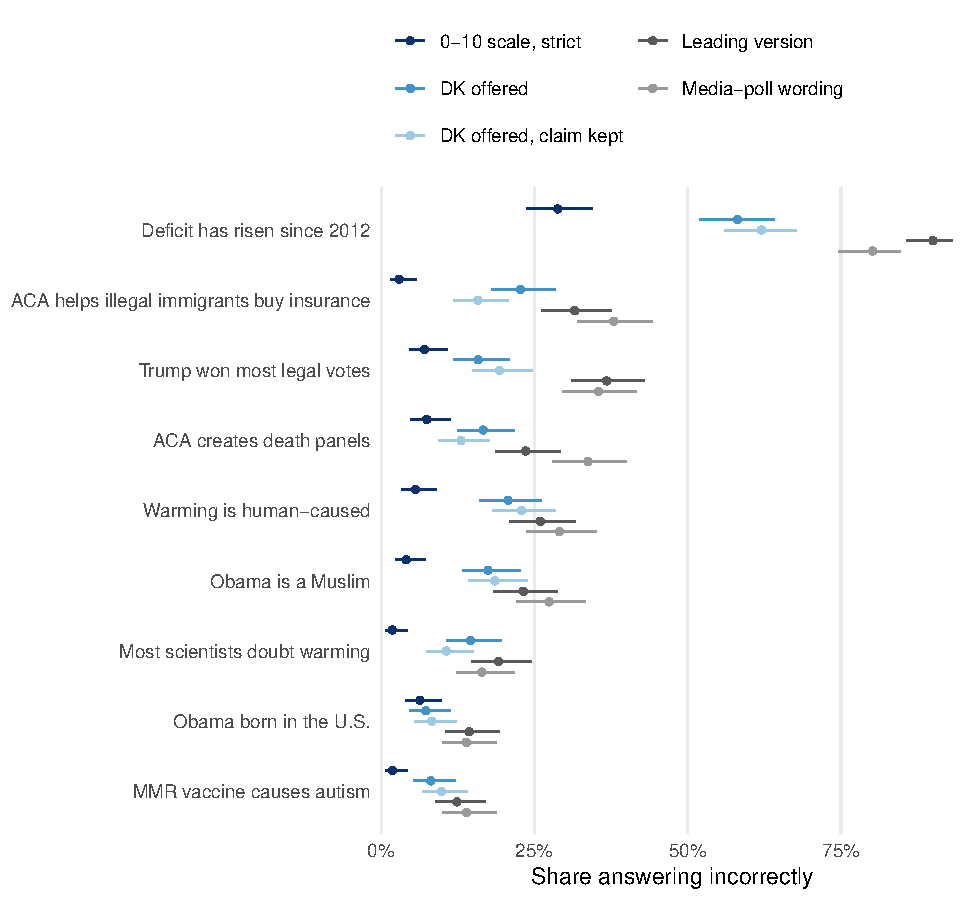
\includegraphics[width=\linewidth]{arms.pdf}
\caption{Share answering incorrectly, by version of the question. Points are shares of the respondents randomly assigned to each version; lines are 95\% Wilson intervals. For multiple choice, the share choosing an incorrect option (DK and skipped answers count as not incorrect); for the 0--10 scale, the share rating the statement at the wrong end (0 for a truth, 10 for a falsehood).}
\label{fig:arms}
\end{figure}

\begin{figure}[t]
\centering
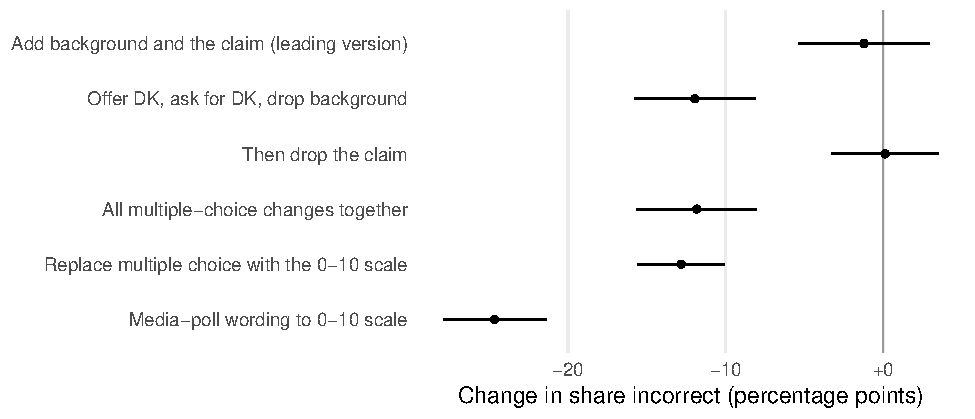
\includegraphics[width=\linewidth]{contrasts.pdf}
\caption{What each design change does. Points are differences in the share answering incorrectly between randomly assigned versions, averaged over the nine questions (a regression of answering incorrectly on version with question fixed effects); lines are 95\% intervals with standard errors clustered by respondent.}
\label{fig:contrasts}
\end{figure}

Figure~\ref{fig:arms} shows the share answering each question incorrectly in each version, and Figure~\ref{fig:contrasts} the average effect of each change. With media-poll wording, \meanMedia{} of answers were incorrect on average. Offering and encouraging DK, and dropping the background, reduced that to \meanFewer{}, by \dkEffect{} points (95\% interval \dkLower{} to \dkUpper{}); respondents in the two DK versions said ``don't know'' to \dkFewer{} and \dkDkOffered{} of the questions. Dropping the false claim from the stem then made no difference (\claimEffect{} points; \claimLower{} to \claimUpper{}), and neither did adding background and the claim to every item (\pyriteEffect{} points relative to media-poll wording; \pyriteLower{} to \pyriteUpper{}). The DK option and the preface that encourages it do the work; the claim in the stem, which one might have expected to lead ignorant respondents astray, does not.

The 0--10 scale finds less misinformation still: \meanScale{} of ratings sat at the wrong end, \scaleEffect{} points below the best multiple-choice version (\scaleLower{} to \scaleUpper{}). From media-poll wording to the scale, estimated misinformation fell by \totalEffect{} points, or by about three-quarters. For Obama's religion, \muslimMedia{} answered ``Muslim'' with media-poll wording, \muslimDk{} with a DK option, and \muslimScale{} were confident of it on the scale; for the ACA and illegal immigrants, the numbers are \illegalMedia{}, \illegalDk{}, and \illegalScale{}.

The deficit item is the exception, and an instructive one. Most respondents in every version said the deficit had risen since 2012 (\deficitMedia{} with media-poll wording, \deficitDk{} with a DK option), and \deficitScale{} were confident of it on the scale. The two versions that told respondents Republicans had held the House since 2012 show \deficitPyrite{} and \deficitFewer{}, against \deficitMedia{} and \deficitDk{} in their counterparts without that cue. Here a falsehood that fits a common stereotype---deficits grow---survives every design change, which suggests that the scale measures misinformation rather than merely suppressing answers.

\FloatBarrier
\section{Discussion}

Poll-based political reporting, long dotted with statistical vignettes suggesting the existence of widespread ignorance (the absence of relevant cognition), now features similar vignettes suggesting the existence of widespread misinformation (the presence of incorrect cognition). Barack Obama is a Muslim. The Affordable Care Act includes ``death panels.'' Has widespread ignorance been replaced with widespread misinformation? The data suggest not. Survey items used to measure misinformation often include features that overstate the extent to which people are misinformed, and the most common of them, the absence of an explicit DK, matters most. That has caused misinformation about misinformation. People are less misinformed than uninformed.

The considerably higher levels of ignorance (and simultaneously, considerably lower levels of misinformation) that we find make sense in light of other facts. On the whole, the American public is politically disinterested and disengaged; in a large sample of web browsing, only about 4\% of users read at least ten news articles and two opinion pieces over three months \citep{flaxman2016}. Misinformation is closer to knowledge in that people generally need to consume political information to walk away with facts or commonly espoused fictions. If people aren't consuming much political information, chances are that they aren't aware of the prominent untruths that underlie many of the claims about a public awash in misinformation.

Furthermore, the case for partisan selective exposure is weaker than first thought \citep{gentzkow2011, prior2013}. If people receive balanced information, they plausibly see both misinformation and corrections. People appear fairly even-handed in how they learn \citep{khanna2018}, and the emerging consensus, displacing earlier evidence \citep{nyhan2010b}, is that corrections mostly succeed \citep{wood2019, guess2020, nyhan2020}. The evidence we present fits what this other research predicts. It also bears on the debate over whether partisan differences in answers to factual questions reflect cheerleading \citep{bullock2015, prior2015, schaffner2018} or sincere belief \citep{berinsky2018}. Using these data among others, \citet{shen2025} find that design features that encourage guessing inflate partisan knowledge gaps by about 40 percent, through the guesses of the ignorant rather than cheerleading.

Even the scale's estimate may be too high. \citet{graham2023} finds that respondents who say they are certain of a falsehood often give a different answer weeks later, which suggests that some confident wrong answers are guesses made on the spot. Our estimates are also from a single convenience sample, and the corpus is limited to items archived by one organization and to topics that had drawn media attention.

Finding that far fewer people are misinformed about the most prominently advocated untruths is not the same as saying that the public is not misinformed about politics. Our data are only about prominent political untruths. It is plausible that people invent a broad variety of political fictions to suit their prejudices and whims and that the net amount of misinformation they hold is much larger. That is a related but separate claim that needs to be studied. Our goal in this paper was narrower---to interrogate the levels of misinformation about common political untruths. The data show that those levels are considerably lower than media polls suggest.

\bibliographystyle{apsr}
\bibliography{references}

\clearpage
\appendix
\section*{Appendix}
\setcounter{table}{0}
\renewcommand{\thetable}{A\arabic{table}}

\begin{table}[H]
\centering
\caption{Media-poll items excluded from the corpus}
\label{tab:exclusions}
\small
\begin{tabular}{p{11cm}r}
\toprule
Reason for exclusion & Items \\
\midrule
Answer not settled when asked, or settled differently later & 27 \\
Open-ended, or asked only of those who did not know & 13 \\
Ambiguous wording, or a key that cannot be verified & 11 \\
Not a factual proposition with one right answer &  8 \\
\bottomrule
\end{tabular}

\begin{minipage}{0.85\linewidth}
\vspace{0.5em}\footnotesize \emph{Note:} Of \nCorpus{} items in the original collection. The replication files give the reason for each item.
\end{minipage}
\end{table}

\begin{table}[H]
\centering
\caption{Media-poll items that let respondents say how sure they were}
\label{tab:graded}
\small
\begin{tabular}{p{8.5cm}lrr}
\toprule
Statement & Fielded & Wrong side & Definitely wrong \\
\midrule
Former President Obama ordered wire taps on Donald Trump's phones & 03/06-07/17 & 30 &  9 \\
Russia hacked the email of Democrats in order to increase the chance that Donald Trump would win the Presidential election. & 06/04-06/17 & 45 & 17 \\
Russia tampered with vote tallies in order to get Donald Trump elected President. & 06/04-06/17 & 38 & 13 \\
Russia hacked the email of Democrats in order to increase the chance that Donald Trump would win the Presidential election. & 05/13-16/17 & 46 & 16 \\
Russia tampered with vote tallies in order to get Donald Trump elected President. & 05/13-16/17 & 35 & 11 \\
Russia hacked the email of Democrats in order to increase the chance that Donald Trump would win the Presidential election. & 07/09-11/17 & 43 & 17 \\
Russia tampered with vote tallies in order to get Donald Trump elected President. & 07/09-11/17 & 40 & 15 \\
Millions of illegal votes were cast in the election. & 06/04-06/17 & 43 & 12 \\
Millions of illegal votes were cast in the election. & 05/13-16/17 & 43 & 10 \\
Millions of illegal votes were cast in the election. & 07/09-11/17 & 46 & 17 \\
\bottomrule
\end{tabular}

\begin{minipage}{0.95\linewidth}
\vspace{0.5em}\footnotesize \emph{Note:} Economist/YouGov polls, 2017, percent of respondents. ``Wrong side'': definitely or probably on the wrong side; ``Definitely wrong'': definitely on the wrong side. The wiretap and vote-tally statements are false; the email-hacking statement is true.
\end{minipage}
\end{table}

\end{document}
